

	\begin{minipage}{\linewidth}
		
		\section{Schwingungen}
		
		\subsection{Eigenfrequenz}
		
%			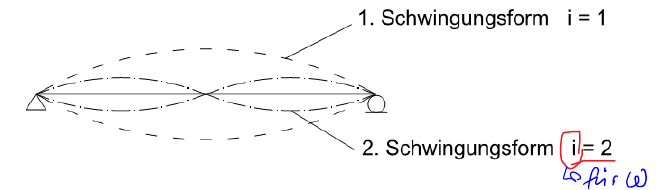
\includegraphics[width=\linewidth]{images/Schwingung1Schwingungsform.PNG}
			
		\begin{tabular}{l|l|p{0.25\linewidth}p{0.3\linewidth}}
			
			\multicolumn{4}{c}{\textbf{Balken mit konstanter Biegesteifigkeit}} \\ \hline
		
			$ f = \frac{\omega}{2 \pi} $ & [Hz][$ \frac{1}{s} $]	& Frequenz	&  \\ \hline
			
			$ \omega = \frac{i^2 \pi^2}{l^2} \sqrt{ \frac{EI}{m} } $ & [ $ \frac{rad}{sec} $ ]	& Kreisfrequenz 	& \multirow{4}{*}{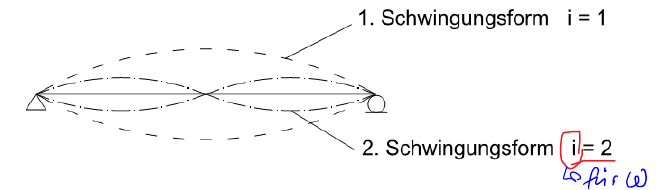
\includegraphics[width=\linewidth]{images/Schwingung1Schwingungsform.PNG} }\\
						&				& i = Schwingungsform 	& \\
						&				& EI = K = Federsteifigkeit & \\ 
						&				& m = Masse pro Längeneinheit $ m = \frac{g [kN/m'] }{9.61 [m/s^2]} $ & \\ \hline
					
					
			\multicolumn{4}{c}{\textbf{Balken mit gleichmässig verteilter Masse}} \\ \hline
				
			$ \omega = \frac{A}{l^2} \sqrt{ \frac{EI}{m} } $ & [ $ \frac{rad}{sec} $ ] & Kreisfrequenz & \\
						&				& A = $ i^2 \cdot \pi^2 $ &   \\ \hline
			
			\multicolumn{4}{c}{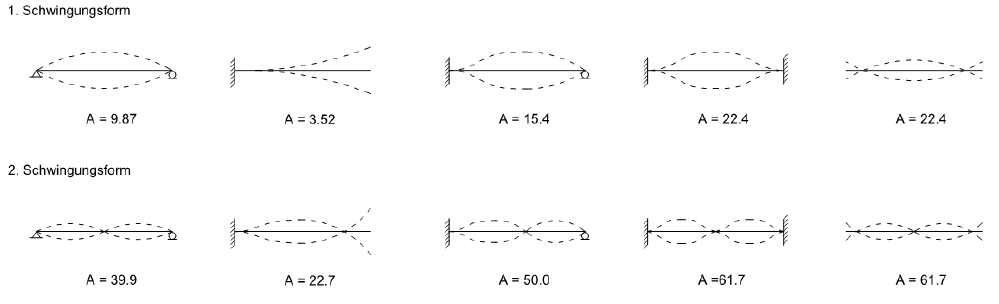
\includegraphics[width=\linewidth]{images/Schwingung2Schwingungsform.PNG} } \\ \hline
			
			\multicolumn{4}{c}{\textbf{Balken mit verteilter Masse und konzentrierter Einzelmasse } } \\ \hline
			
			\multicolumn{4}{c}{ 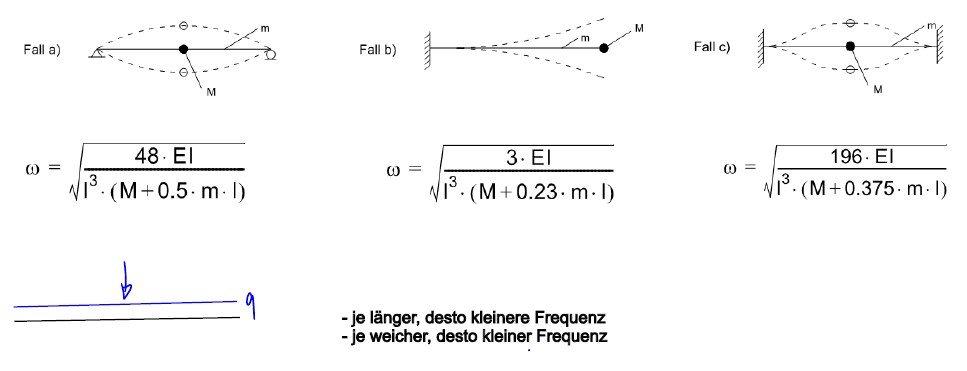
\includegraphics[width=0.8\linewidth]{images/Schwingung3Schwingungsform.PNG} } \\ \hline
		
		\end{tabular}
		
	\end{minipage}
	\begin{minipage}{0.5\linewidth}
		
		\begin{itemize}
			\item + Eigenfrequenz, je mehr Freiheitsgrade der Auflager blockiert
			
			\item Systemlänge geht quadratisch ein $ \rightarrow $ Verkürzung des Systems = höhere Eigenfrequenz
			
			\item Biegesteifigkeit geht als Wurzel ein $ \rightarrow $ höhere Biegesteifigkeit EI = nur kleine Erhöhung der Eigenfrequenz
			
		\end{itemize}
		
	\end{minipage}